\documentclass[12pt,final,oneside]{article} % use larger type; default would be 10pt
\usepackage{etex}
\usepackage[utf8]{inputenc} % set input encoding (not needed with XeLaTeX)
\usepackage[margin=2cm]{geometry}
\usepackage{xy}
\usepackage{amsmath, amsthm}
\usepackage{showkeys}
\usepackage[smaller]{acronym}
\usepackage[marginclue]{fixme}
%\usepackage{natbib}
\usepackage{tabularx}
\usepackage{chngpage}
\usepackage{booktabs}
\usepackage{cite}
\usepackage{times}
\usepackage{graphicx}
\usepackage{ctable}
\usepackage{footnote}
\usepackage{amssymb}
\usepackage{url}
\usepackage{tikz-timing}
\usepackage[lofdepth,lotdepth]{subfig}
\usepackage{multirow}
\usepackage{tameflts}
\usepackage{algpseudocode}
\usepackage{algorithm}
\usepackage{placeins}
\usepackage{hyperref}
\fxsetup{
    status=draft,
    author=,
    layout=marginclue,inline, % also try footnote or pdfnote
    theme=color
}
\definecolor{fxnote}{rgb}{0.8000,0.0000,0.0000}

\setcounter{tocdepth}{3}

\usepackage{color}
\usepackage[final]{listings}
\lstset{ %
language=C++,                % choose the language of the code
basicstyle=\ttfamily,       % the size of the fonts that are used for the code
numbers=left,                   % where to put the line-numbers
numberstyle=\footnotesize,      % the size of the fonts that are used for the line-numbers
stepnumber=1,                   % the step between two line-numbers. If it is 1 each line will be numbered
numbersep=5pt,                  % how far the line-numbers are from the code
backgroundcolor=\color{white},  % choose the background color. You must add \usepackage{color}
showspaces=false,               % show spaces adding particular underscores
showstringspaces=false,         % underline spaces within strings
showtabs=false,                 % show tabs within strings adding particular underscores
frame=single,           % adds a frame around the code
tabsize=2,          % sets default tabsize to 2 spaces
captionpos=b,           % sets the caption-position to bottom
breaklines=false,        % sets automatic line breaking
breakatwhitespace=false,    % sets if automatic breaks should only happen at whitespace
escapeinside={\%*}{*)}          % if you want to add a comment within your code
}
\begin{document}

\section{Data Structures}\label{secDatastructures}
\subsection{Basic Types}
The following are the basic types, out of which others are built, and which will be referred to. There is generally, but not always, a direct relationship to a C++ primitive.
\\
        \begin{tabularx}{\linewidth}{XXX}
        \toprule
        Name & Closest C++ Equivalent & Description\\
        \midrule
        Integer &  int & Whole number \\
        Float & float & Floating point number \\
        Queue & std::list & FIFO queue \\
        List(type) & std::list$\langle$type$\rangle$ & \\
        String & std::string & String object that provides operations to manipulate itself \\
        File & std::iostream & Abstract type to represent simple I/O operations \\
        Map(KeyType $\to$ ValueType, DEFAULT:  DefaultValue) & std::unordered\_map$\langle$KeyType, ValueType$\rangle$ &  A map to translate values of type KeyType to values of type ValueType. If the key isn't present, returns DefaultValue \\
        \bottomrule
        \end{tabularx}
\\
\\
The following are complex types, which are further defined below. This is merely a quick description of each.
\\
        \begin{tabularx}{\linewidth}{lX}
        \toprule
        Name & Description\\
        \midrule
        Blif & Parent object, contains all information about a BLIF file and provides useful operations \\
        Model & Represents a circuit within a BLIF file, and provides methods to manipulate said circuit \\
        BlifNode & A circuit element, or node in the DFG representing the circuit \\
        Signal & A signal within a specific circuit, or Model, representing a set of edges with common source \\
        \bottomrule
        \end{tabularx}

   \begin{figure}
      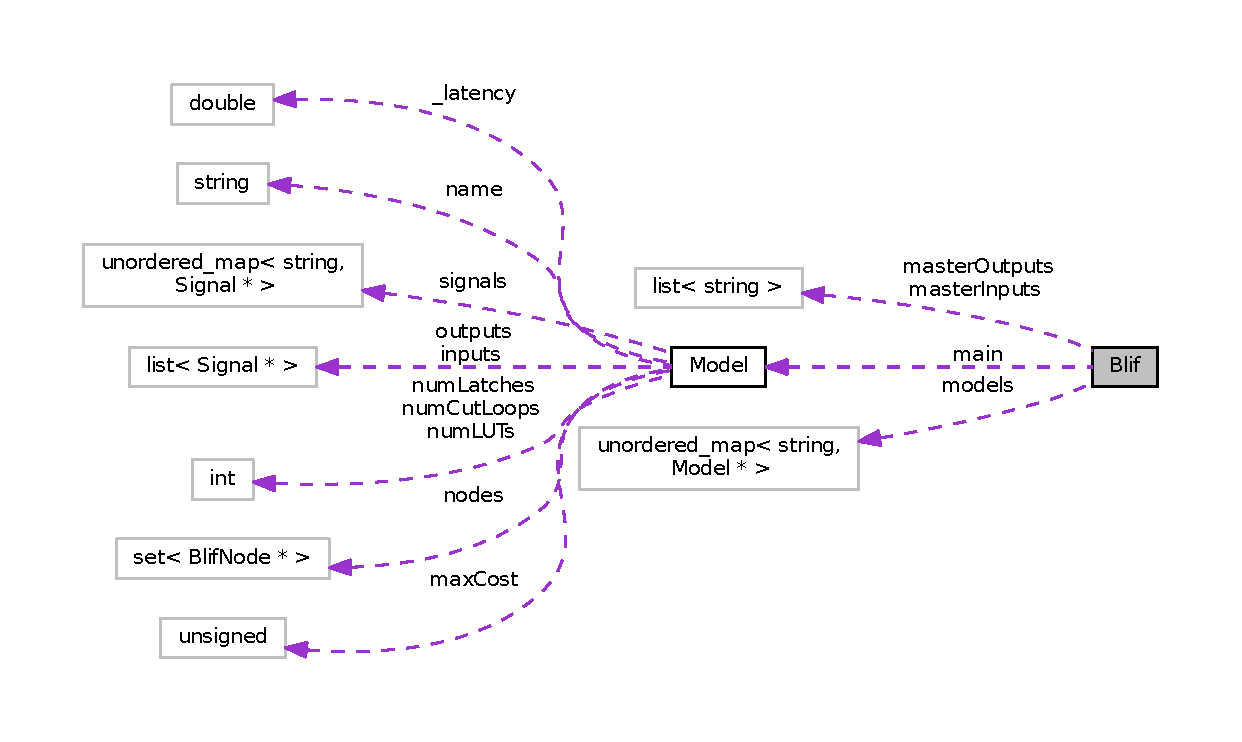
\includegraphics{doxygen/classBlif__coll__graph.pdf}
   \end{figure}
   \begin{figure}
      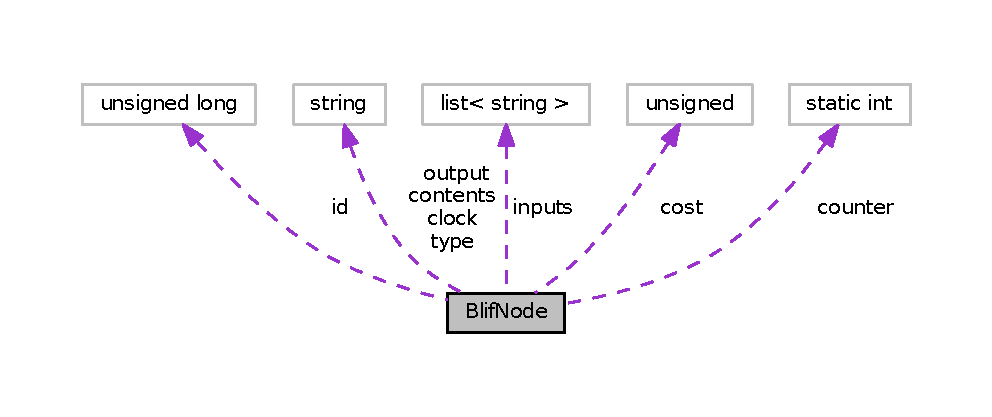
\includegraphics{doxygen/classBlifNode__coll__graph.pdf}
   \end{figure}
   \begin{figure}
      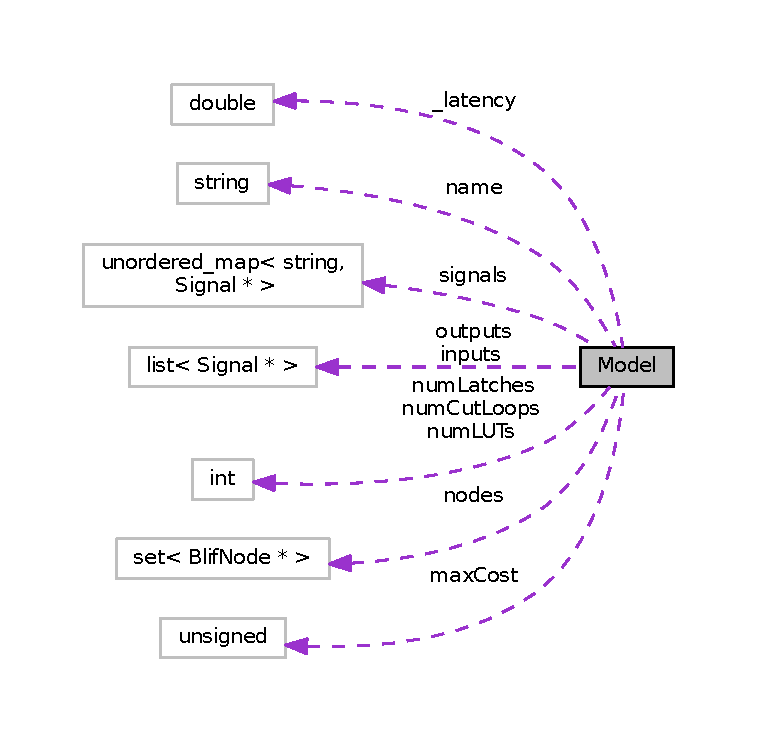
\includegraphics{doxygen/classModel__coll__graph.pdf}
   \end{figure}
   \begin{figure}
      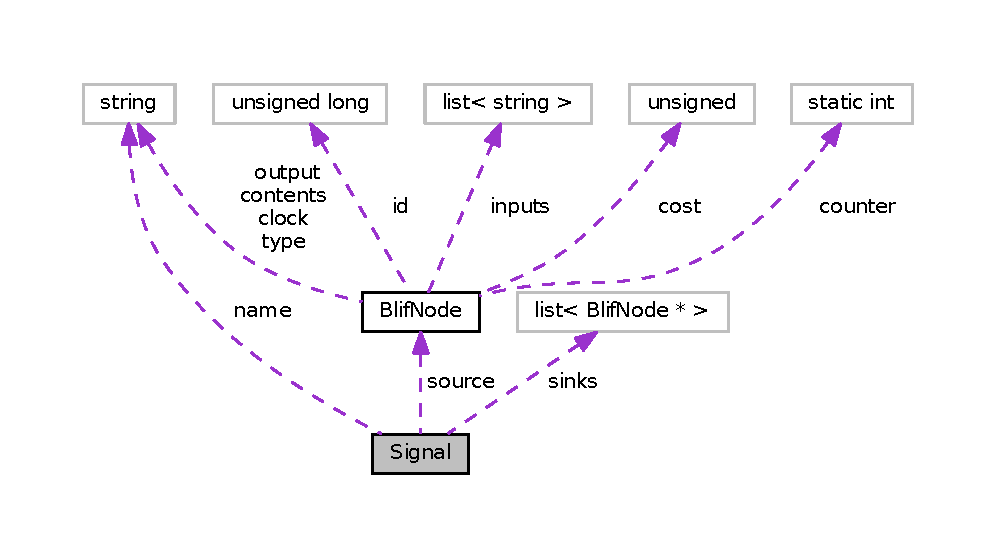
\includegraphics{doxygen/classSignal__coll__graph.pdf}
   \end{figure}

   \subsection{Blif}
      
   \subsection{Model}
      Represents the circuit as a DFG. Contains a list of nodes, map of signal name $\to$ Signal*, and lists of primary inputs and outputs for the circuit.
      Each node contains the names of its input and output signals, allowing the Signal* to be looked up, then the Signal* contains pointers to its source and sink nodes.
      This allows the DFG to be traversed by going from node, to signal, to node, etc.
      A BlifNode represents the information in a circuit element declaration within a \ac{BLIF} file, which includes only the name of its input and output signals. The actual Signal itself is a separate circuit specific construct designed to allow for ease of traversal of the circuit as a \ac{DFG}.
      As such, we don't directly point to signals from a BlifNode, as the Signal depends on the circuit context.
      \fixme{TODO: Image showing DFG traversal, and example of blif file and class contents}

\newpage
\section{Algorithm}
Types marked with an * are custom types defined previously in section \ref{secDatastructures}.
\subsection{Main}
Partition, Triplicate, Join and Flatten are all implemented in separate programs. Main is responsible for taking an input file and running it through our toolchain to produce a TMR'd output file.
\begin{algorithm}
    \begin{center}
        \begin{tabular}{lll}
        \toprule
        Variable & Type & Description\\
        \midrule
        $input$ & \bf{File} & Input blif file\\
        $targetRecoveryTime$ & \bf{float} & Per partition recovery time (in seconds) \\
        $files$ & \bf{List(File)} & circuit partitions, one per file \\
        $file$ & \bf{File} & \\
        $header$ & \bf{string} & string containing the first three lines of the input file \\
        $output$ & \bf{File} & output file\\
        \bottomrule
        \end{tabular}
    \end{center}
   \caption{Main Algorithm}\label{main}
   \begin{algorithmic}[1]
      \Procedure{Main}{$input$, $targetRecoveryTime$}
         \State $files \gets \mbox{Partition}(input)$
         \ForAll {$file \in files$}
            \State $file \gets \mbox{Triplicate}(file)$
         \EndFor
         \State $header \gets input.lines[0\to 3]$
         \State $file \gets \mbox{Join}(files, header)$
         \State $output \gets \mbox{Flatten}(output)$
      \EndProcedure
   \end{algorithmic}
\end{algorithm}
We're given a blif file as input.
In line 11 we partition the input circuit into a number of sub circuits, each in a separate file, as further expanded in Algorithm \ref{partition}.
Then in lines 12-13 for each partition file, we read it in as a black box, triplicate it, insert voting logic, and write it back out.
Next in line 14 we extract the original header, which provides the name, inputs and outputs of the original circuit.
We then, in line 15, join all the partitions together with the original name, inputs and outputs (in the same order), as the original circuit, and finally line 16 flattens the circuit, i.e. transforms the generated heirarchical netlist into a flat netlist with only one main model, or circuit, and no submodels.

\newpage
\subsection{Partition}
Given an input file, Partition reads it in, and splits it into a number of smaller subcircuits, each of which has a maximum recovery time of our target recovery time or less. Each subcircuit is then output to its own separate file, each of which is a valid \ac{BLIF} and circuit on its own.
\begin{table}
    \begin{center}
        \begin{tabularx}{\linewidth}{llX}
        \toprule
        Variable & Type & Description\\
        \midrule
        $file$ &\bf File  & input file\\
        $targetRecoveryTime$ &\bf  float & maximum per partition recovery time (in seconds)\\
        $blif$ &\bf  Blif* & In-memory representation of input blif file\\
        $circuit$ &\bf   Model* & Main circuit from input file, represented as DFG\\
        $partition$ &\bf   Model* & Circuit, which we are adding nodes to, to make our partition\\
        $queue$ &\bf  Queue & FIFO queue of nodes to visit\\
        $visited$ &\bf   Map(BlifNode*$\to$ bool)& Map of whether a BlifNode is visited\\
        $signal$ &\bf  Signal* & \\
        $circuit.outputs$ &\bf  List(Signal*) & List of output Signal* of a circuit\\
        $signal.source$ &\bf  BlifNode* & Node which drives this Signal*\\
        $queue.size$ &\bf  integer & Number of nodes in queue\\
        $node$ &\bf  BlifNode* & \\
        $file$ &\bf  File & \\
        $files$ &\bf  List(File) & \\
        $numPartitions$ &\bf  int & Counter of number of partitions\\
        $signalName$ &\bf  string & Name of a Signal*\\
        $node.inputs$ &\bf  List(string) & List of names of signals which are inputs to this node\\
        $model.signals$ &\bf  Map(string $\to$ Signal*) & Map from signal name to Signal* representing it in that Model*\\
        \bottomrule
        \end{tabularx}
        \caption{Variables for Partition}
        \label{varPart}
    \end{center}
\end{table}
\begin{algorithm}
   \caption{Partition}\label{partition}
   \begin{algorithmic}[1]
         \Procedure{Partition}{$file$}
            \State $blif \gets$ new Blif(file) \Comment{Read in $file$}
            \State $circuit \gets blif.main$ \Comment{The actual circuit within the blif file}
            \State $partition \gets$ new Model \Comment{Empty Circuit}
            \State $queue \gets$ new Queue \Comment{Empty Queue}
            \State $visited \gets$ new Map(BlifNode $\to$ bool, DEFAULT: false)

            \ForAll{$signal \in circuit.outputs$}
               \State $queue.\mbox{Enqueue}(signal.source)$
            \EndFor

            \While{$queue.size > 0$}
               \State $node \gets queue.\mbox{Dequeue()}$
               \If{$visited[node] = $ true}
                  \State continue \Comment{Handle each node once and only once}
               \EndIf
               \State $visited[node] \gets $ true
               \State $partition.\mbox{AddNode}(node)$
               \If{$partition.\mbox{RecoveryTime}() > targetRecoveryTime$}
                  \State $partition.\mbox{RemoveNode}(node)$
                  \State MakeIOList$(partition, circuit)$
                  \State $file \gets partition.\mbox{WriteToFile}()$
                  \State $files \gets files+file$
                  \State $numPartitions \gets numPartitions+1$
                  \State $partition \gets$ new Model \Comment{Empty Circuit}
                  \State $partition.\mbox{AddNode}(node)$
               \EndIf
               \ForAll{$signalName \in node.inputs$}
                  \State $signal \gets model.signals[signalName]$
                  \State $queue.\mbox{Enqueue}(signal)$
               \EndFor
            \EndWhile
            \If{$partition.size > 0$}
               \State MakeIOList$(partition, circuit)$
               \State $file \gets partition.\mbox{WriteToFile}()$
               \State $files \gets files+file$
            \EndIf
            \State return $files$
         \EndProcedure
   \end{algorithmic}
\end{algorithm}
\FloatBarrier
Line 2 reads a \ac{BLIF} into memory, transforming from the \ac{BLIF} format described in \fxfatal{TODO: Reference} to the one represented by \fxfatal{TODO: Reference}.
Lines 12-15 ensure that we visit each node only once, and thus that each node is in exactly one partition, by checking if a node has been visited before and if so, skipping it, otherwise marking it as visited and coontinuing.
Lines 16/24 inserts the current node into the open partition, cutting any created cycles and updating values such as critical path length as outlined in Algorithm \ref{addnode}.
Line 17 tests if the current partition recovery time is greater than our specified limit, with the algorithm used to calculate the recovery time located at Algorithm \ref{recoverytime}.
If the recovery time is greater we execute lines 18-24, where we remove the just added node to bring our recovery time back under the limit, and then write the partition to a file.
Line 18 calculates which signals are primary inputs or outputs for the partition, and promotes them accordingly, with more detail given in Algorithm \ref{makeiolist}.
Writing the partition to a file simply involves outputting the name, inputs, outputs, and a list of every node in the partition in \ac{BLIF} format.
RemoveNode, on line 19, merely removes the node from the partition's list of nodes rather than fully reversing everything AddNode does. As WriteToFile simply serialises the inputs, outputs and node list this is all that's required with the caveat that some cycles may be cut unecessarily.
Lines 31-34 write out the final partially full partition, if there is one. Again, WriteToFile simply outputs the circuit name, list of inputs, outputs and clocks, and list of nodes, with no further processing required.


\newpage
\subsection{MakeIOList}
Given an original partition and a subpartition, promote any signals which are sourced or sunk outside of the subpartition to a primary input or output of the subpartition.
\begin{algorithm}
   \begin{center}
        \begin{tabularx}{\linewidth}{llX}
        \toprule
        Variable & Type & Description\\
        \midrule
        $partition$ &\bf  Model* & Partition to create list of primary inputs and outputs for\\
        $originalCircuit$ &\bf  Model* & Original model \\
        $signal$ &\bf  Signal* & \\
        $signal.source$ &\bf  BlifNode* & The driver for the signal \\
        $partition.inputs$ &\bf  List(BlifNode*) & List of primary inputs for the circuit \\
        $partition.signals$ &\bf  Map(string $\to$ Signal*) & Map from signal name to Signal* \\
        $originalCircuit.signals$ &\bf  Map(string $\to$ Signal*) & Map from signal name to Signal* \\
        $signal.sinks$ &\bf  List(BlifNode*) & List of sinks for the signal \\

        \bottomrule
        \end{tabularx}
    \end{center}
   \caption{MakeIOList}\label{makeiolist}
   \begin{algorithmic}[1]
         \Procedure{MakeIOList}{$partition, originalCircuit$}
            \ForAll{$signal \in partition.signals$}
               \If{$signal.source = NULL$} \Comment{If this signal has no driver}
                  \State{$partition.inputs.Add(signal)$}
               \EndIf
               \State $otherSignal \gets originalCircuit.signals[signal.name]$ \Comment{Get the corresponding signal in the original circuit}
               \If{$otherSignal.sinks - signal.sinks > 0$} \Comment{If the signal has more sinks in the original circuit than it does in this partition}
                  \State $partition.outputs.Add(signal)$
               \EndIf
            \EndFor
         \EndProcedure
   \end{algorithmic}
\end{algorithm}
We iterate through every signal in our partition. For each one we check if we have a source (line 4), if not it must be a primary input. Similarly, on line 7 we check if we have a sink which is not represented within our partition. If so, promote it to a primary output of the partition.


\newpage
\subsection{RecoveryTime}
For a given partition, calculate its error recovery time.
\begin{algorithm}
   \begin{center}
        \begin{tabularx}{\linewidth}{llX}
        \toprule
        Variable & Type & Description\\
        \midrule
        $latency$ &\bf  float & Circuit latency (i.e. time for input to completely propagate to output) in seconds\\
        $clockFrequency$ &\bf  Integer & Operating frequency of the circuit, in seconds\\
        $criticalPath$ &\bf  Integer & Maximum number of steps between an input and an output\\
        $numFF$ &\bf  Integer & Number of Latches in circuit\\
        $numLUT$ &\bf  Integer & Number of look up tables in circuit\\
        $resynchronisationTime$ &\bf  Float & Time, in seconds, that it takes to resynchronise circuit\\
        $detectionTime$ &\bf  Float & Time, in seconds, that it takes to detect an error\\
        $ReconfigureTime$ &\bf  Float & Time, in seconds, that it takes to reconfigure circuit\\
        $communicationTime$ &\bf  Float & Time, in seconds, that it takes to transmit reconfiguration request to controller\\
        \bottomrule
        \end{tabularx}
    \end{center}
   \caption{RecoveryTime}\label{recoverytime}
   \begin{algorithmic}[1]
         \Procedure{RecoveryTime}{$partition$}
            \State $latency \gets frequency\times{}(criticalpath+1)$
            \State $detectionTime \gets latency$
            \State $resynchronisationTime \gets latency$
            \State $reconfigurationTime \gets \mbox{max}(numFF, numLUT)/10/15...more stuff$
            \State $communicationTime \gets numPartitions\times{}latency\times{}more stuff$
            \State $recoveryTime \gets detectionTime+resynchronisationTime+reconfigurationTime+communicationTime$
            \State return $recoveryTime$
         \EndProcedure
   \end{algorithmic}
\end{algorithm}
The derivation of this algorithm and the values used is fully discussed in Section \fxfatal{TODO: Reference}. The criticalpath is a measure of the maximum number of latches on a path from input to output. The +1 is to account for the contribution of combinational logic, which may be up to one additional clock cycle of latency.


\newpage
\subsection{AddNode}
Insert a node into an existing partition, or circuit, while updating appropriate parameters (i.e. maximum path length and signals) which are depended upon by other components (i.e. recovery time calculation and \ac{DFG} traversal respectively).
Additionally, detect any newly created cycles and cut them.
This ensures that the circuit is always (except within this method) an acyclic graph with every node reachable.
\begin{algorithm}
    \begin{center}
        \begin{tabularx}{\linewidth}{llX}
        \toprule
        Variable & Type & Description\\
        \midrule
        $partition$ &\bf  Model* & Model* containing DFG representing partition to add node to\\
        $node$ &\bf  BlifNode* & Node to add\\
        $signal$ &\bf  Signal* & \\
        $signalName$ &\bf  string & \\
        $partition.cutLoops$ &\bf  Map[string $\to$ string] & For signals which have been cut, a map of the old to the new name\\
        $partition.signals$ &\bf  Map[string $\to$ Signal* & Map of signal name to Signal* \\
        $signal.sinks$ &\bf  List(BlifNode*) & List of sinks for a Signal* \\
        $signal.source$ &\bf  BlifNode* & Source, or driver, for a Signal* \\
        $inCost$ &\bf  int & Maximum number of critical path steps to reach node, not counting the node itself \\
        $explored$ &\bf  Map(BlifNode* $\to$ boolean) & Whether a node has been reached yet in the current iteration \\ 
        \bottomrule
        \end{tabularx}
    \end{center}
   \caption{AddNode}\label{addnode}
   \begin{algorithmic}[1]
         \Procedure{AddNode}{$partition, node$}
            \State $nodes.insert(node)$
            \ForAll{$signalName in node.inputs$}
               \If{$partition.cutLoops[signalName] \neq ""$}
                  \State $signalName \gets cutLoops[signalName]$ \Comment{If this signal has been renamed already to avoid a cycle, rename this occurance of it.}
               \EndIf
               \State $signal \gets partition.signals[name]$
               \State $signal.sinks.Add(node)$
            \EndFor
            \State $signal \gets partition.signals[node.output]$
            \State $signal.source \gets node$

            \State $inCost \gets 0$
            \ForAll{$signalName \in node.inputs$}
               \State $source \gets partition.signals[signalName].source$
               \If{$partition.costs[source] > inCost$}
                  \State $inCost \gets partition.costs[source]$
               \EndIf
            \EndFor
            \State UpdateCostsAndBreakCycles$(partition, node, NULL, node, inCost, explored, costs)$
         \EndProcedure
   \end{algorithmic}
\end{algorithm}
Lines 4-6 check if one of the inputs signals for this node has been cut to remove a cycle. If so, we rename the signal appropriately, to what the new primary input is called.
Additionally, lines 3-11 update the appropriate signals so that this node is reachable within the \ac{DFG}.
Lines 12-19 then update the maximum path length (or latency in clock cycles) while detecting and cutting any newly created cycles.


\newpage
\subsection{UpdateCostsAndBreakCycles}
Recursively traverse our network to update maximum path lengths to account for our new node and additional paths. While traversing the network, detect and break any cycles we encounter.
This turns a possibly cyclic \ac{DFG} with partially computed path lengths, into an acyclic \ac{DFG} with fully computed path lengths.

\begin{algorithm}
    \begin{center}
        \begin{tabularx}{\linewidth}{llX}
        \toprule
        Variable & Type & Description\\
        \midrule
        $partition$ &\bf  Model* & Model* containing DFG representing partition to add node to\\
        $root$ &\bf  BlifNode* & Newly added node\\
        $node$ &\bf  BlifNode* & Node we just came from\\
        $node$ &\bf  BlifNode* & Current node\\
        $costToReach$ &\bf  int & Maximum number of critical path steps to reach node, not counting the node itself \\
        $explored$ &\bf  Map(BlifNode* $\to$ boolean) & Whether a node has been reached yet in the current iteration \\ 
        $partition.signals$ &\bf  Map[string $\to$ Signal* & Map of signal name to Signal* \\
        $partition.signals[parent.output]$ &\bf  BlifNode* & Signal driven by the prior node i.e. the graph edge we most recently travelled. \\
        $node.cost$ &\bf  int & 1 for latches, 0 for LUTs \\
        $costs$ &\bf  Map(BlifNode* $\to$ int) & Map of the cost to reach each node \\
        $node$ &\bf  BlifNode* & \\
        $signal.sinks$ &\bf  List(BlifNode*) & List of sinks for a Signal* \\
        $cost$ &\bf  int & Number of critical path steps to reach node, including the node itself \\
        \bottomrule
        \end{tabularx}
    \end{center}
   \caption{UpdateCostsAndBreakCycles}\label{updatecosts}
   \begin{algorithmic}[1]
      \Procedure{UpdateCostsAndBreakCycles}{$partition, root, parent, node, costToReach, explored$}
      \If{$explored[node] = true $ and $costs[node] \ge costToReach$} \Comment{Already expanded this path, and it can't change}
            \State return
         \EndIf
         \If{$parent \neq NULL $ and $ node = root$} \Comment{We have a cycle, as all newly created cycles must go through the new node, and the new node should only ever be reached once at the start without cycles}
            \State CutSignal$(partition, partition.signals[parent.output])$
            \State return
         \EndIf
         \State $cost \gets costToReach+node.cost$
         \If{$cost > costs[node]$}
            \State $costs[node] = cost$
         \Else
            \State $cost = costs[node]$
         \EndIf
         \ForAll{$node \in partition.signals[node.output].sinks$}
            \State UpdateCostsAndBreakCycles$(root, node, child, cost, explored)$
         \EndFor
         \State $explored[node] = true$
      \EndProcedure
   \end{algorithmic}
\end{algorithm}
We care about two things. One, the maximum cost to reach a node, and two, detecting and removing any cycles.
Given an existing \ac{DAG} \fxnote{Directed Acyclic Graph} which we insert a new node into, then 1. The new node is the root node of a subtree within the \ac{DAG}. 2. Nodes which are not within the subtree cannot have the maximum cost to reach them change (as nothing has changed in any path to them). 3. Any cycles must pass through the new root node, as there are no cycles elsewhere in the graph. 4. Without any cycles, the root node will only be reached once at the start.
Using this information we develop our traversal algorithm.
Line 2 demonstrates an optimisation, in that once a path has been checked we need not recheck it unless we have found a more expensive path to it as otherwise nothing will change.
Lines 5-8 check if we have detected a cycle. If so, cut it through cutting the signal, detailed in algorithm \ref{cutsignal}.


\newpage
\subsection{CutSignal}
Given a signal, cut it, by splitting it into two signals. One of which is a primary input with the sinks of the previous signal. One of which is a primary output with the source of the previous signal.

\begin{algorithm}
    \begin{center}
        \begin{tabularx}{\linewidth}{llX}
        \toprule
        Variable & Type & Description\\
        \midrule
        $partition$ &\bf  Model* & Model* containing DFG representing partition to add node to\\
        $partition.cutLoops$ &\bf  Map(string $\to$ string) & Map from old to new name of a cut signal. Note that only the input signal is renamed. The output signal retains the same name.\\
        $signal$ &\bf  Signal* & The signal we're cutting\\
        $newSignal$ &\bf  Signal* & The new signal we created\\
        $signal.source$ &\bf  BlifNode* & The source, or driver, of a signal\\
        $partition.signals$ &\bf  Map(string $\to$ Signal*) & A map from signal name to signal\\
        $partition.outputs$ &\bf  List(Signal*) & The primary outputs for the circuit\\
        $node$ &\bf  BlifNode* & \\
        $node.inputs$ &\bf  List(string) & names of input signals to a node\\
        \bottomrule
        \end{tabularx}
    \end{center}
   \caption{CutSignal}\label{cutsignal}
   \begin{algorithmic}[1]
      \Procedure{CutSignal}{$partition, signal$}
         \State $newSignal \gets new Signal(name)$ \Comment{Create a new signal with the same name, but currently no sources or sinks}
         \State $newSignal.source \gets signal.source$
         \State $partition.signals[name] \gets newSignal$
         \State replace$(partition.outputs, signal, newSignal)$ \Comment{Replace any occurances of the old signal in the circuit outputs with the new}
         \State $signal.name \gets "qqrin"+name$
         \State $signal.source = NULL$
         \State $signals[signal.name] \gets signal$
         \State $cutLoops[newSignal.name] \gets signal.name$
         \ForAll{$node \in signal.sinks$}
            \State replace$(node.inputs, name, "qqrin"+name)$
         \EndFor
      \EndProcedure
   \end{algorithmic}
\end{algorithm}
Cutting a signal consists of splitting an existing signal into two. One with the same source but no sinks as a primary output. One with the same sinks but no source as a primary input. We also need to update existing references to point to the correct signal, and record the change to update any future references as nodes get added.
To that end, lines 3-5 create a new signal with the same source, no sinks, and replace all existing instances with the new signal.
We now in lines 6-12 rename the previous signal to a reserved name, set it to have no source, and update all its sinks to refer to the correct, renamed signal.

\newpage
\subsection{TMR}
Given a file containing a partition, read it in as a black box, triplicate it, add voter logic, write back out to file.


\begin{algorithm}
    \begin{center}
        \begin{tabularx}{\linewidth}{llX}
        \toprule
        Variable & Type & Description\\
        \midrule
        $file$ &\bf  File & File to triplicate\\
        $circuit$ &\bf  string & Contents of the circuit file\\
        $header$ &\bf  string & String containing the circuit name, inputs and outputs as they appear in the \ac{BLIF}\\
        $voter$ &\bf  string & Contents of the voter circuit file\\
        $subcktDefintionN$ &\bf  string & String representing a subcircuit in \ac{BLIF} format\\
        $voterDefintionN$ &\bf  string & String representing a subcircuit in \ac{BLIF} format\\
        \bottomrule
        \end{tabularx}
    \end{center}
   \caption{TMR}\label{TMR}
   \begin{algorithmic}[1]
      \Procedure{TMR}{$file$}
         \State $circuit \gets file.read()$
         \State $header \gets circuit.header$
         \State $voter \gets voter.read()$
         \State $subcktDefinition1 \gets MakeSubcktDefinition(circuit)$
         \State $subcktDefinition2 \gets MakeSubcktDefinition(circuit)$
         \State $subcktDefinition3 \gets MakeSubcktDefinition(circuit)$
         \State $voterDefinition \gets MakeSubcktDefinition(voter)$
         \State $subcktDefinition.ConnectInputs(circuit.inputs)$
         \State $voterDefinition.ConnectInputs(subcktDefinition1.outputs, subcktDefinition2.outputs, subcktDefinition3.outputs)$ \Comment{Connect the outputs of the partitions to the inputs of the voter}
         \State $voterDefinition.ConnectOutputs(circuit.outputs)$
         \State $file.write(header)$
         \State $file.write(voterDefinition)$
         \State $file.write(subcktDefinition1)$
         \State $file.write(subcktDefinition2)$
         \State $file.write(subcktDefinition3)$
         \State $file.write(voter)$
         \State $file.write(circuit)$
      \EndProcedure
   \end{algorithmic}
\end{algorithm}
This method operates on the \ac{BLIF} in a low level way, dealing manipulating the actual file contents, rather than operating on an abstract circuit representation, as we transform a flat circuit, into a heirarchical circuit, in which out original flat circuit remains untouched but we insert voting and similar logic around it.
We read in our partition circuit and voter circuit. We now create three partition subcircuit and one voter subcircuit definitions. We match up our signal names between them appropriately, and then write out our subcircuit definitions, followed by our partition and voter subcircuits.

This transforms a file from format:
\begin{lstlisting}
.name partition
.inputs ...
contents
\end{lstlisting}
Into one in format:
\begin{lstlisting}
.name TMR
.inputs ...
.subckt partition
.subckt partition
.subckt partition
.subckt voter
.end

.name voter
...
.end
.name partition
...
.end
\end{lstlisting}

\newpage
\subsection{BlifJoin}
Given a list of blif files, concatenates them all together, creates
subcircuit definitions to connect them all together, and writes them to a file

This transforms a set of files in format:
\begin{lstlisting}
.name partitionN
.inputs ...
contents
\end{lstlisting}
Into one file with format:
\begin{lstlisting}
.name TMR
.inputs ...
.subckt partition1
.subckt partition2
.subckt partition3
...
.end

.name partition1
...
.end
.name partition2
...
.end
...
\end{lstlisting}
\newpage
\subsection{Flatten}
Given a heirarchical blif file, run it through abc to flatten it, and postprocess if necessary.
\begin{algorithm}
    \begin{center}
        \begin{tabularx}{\linewidth}{llX}
        \toprule
        Variable & Type & Description\\
        \midrule
        $file$ &\bf  File & File to flatten\\
        \bottomrule
        \end{tabularx}
    \end{center}
   \caption{Flatten}\label{Flatten}
   \begin{algorithmic}[1]
      \Procedure{Flatten}{$file$}
         \Comment{Flattening is currently performed by abc (link), called with parameters:}
         \State ./abc -o output -c echo file
         \Comment{Due to bug in abc, clock information is stripped from latches, so we then call grep and sed to fix the output file}
         \State $latch \gets $split(grep -m 1 '\.latch' file)
         \If{$latch$}
            \State sed -ri 's/(\textbackslash.latch.+)(2)/\textbackslash1 '+latch[3] + ' ' + latch[4] + ' 2/' output
         \EndIf
      \EndProcedure
   \end{algorithmic}
\end{algorithm}

./abc is provided an input file, given the command to echo the current file,
and told to output everything to output.
grep is called to search for latches, and return the latch information if
there is one. If there is, replace the faulty latch information with the
correct information.
This assumes that there is only one global clock, all latches are triggered on
the same signal (e.g. rising edge, falling etc), and all latches have initial
state don't care, which holds true for all provided benchmarks.
\end{document}



      %BEGIN Model->CutLoopsRecursive(state, parent, signal)
         %Variables:
            %state - map of whether a node is explored or not
            %parent - parent node
            %signal - edge into this node
            %node - BlifNode
            %sig - Signal
         %Constants:
            %NEW - 0
            %EXPLORING - 1
            %FINISHED - 2
         %node = signal->source
         %IF(state[node] == EXPLORING) //Found a cycle
            %ReplaceSignalName(parent->inputs, signal->name, "qqrin"+signal->name)
         %ELSEIF(state[node] == FINISHED) //Already explored this path
            %return;
         %ELSE
            %state[node] = EXPLORING
            %FOREACH(sig in node->inputs)
               %this->CutLoopsRecursive(state, node, signal)

         %state[node] = FINISHED
      %END Model->CutLoopsRecursive
%Line 12 tests if we've detected a cycle, through coming across a node marked as EXPLORING, since that means it's an ancestor of this node.
%If so, then in line 13 we rename the input signal to cut the loop. As the input has no source, it automatically gets promoted to primary input.
%If it's not a cycle, then line 14 tests if we've already checked for loops down this path. Since if we have it's a waste of time exploring it again, so we just quit early out of this branch.
%next, in like 17-19 we mark our current node as EXPLORING, and foreach input, recursively expand each.
%Then finally, in line 21, after we've explored all child branches, we can mark this node as FINISHED and return back up the stack.
%Eventually, every node will be marked as FINISHED, and then we have detected and cut all loops in this circuit.

      %BEGIN ReplaceSignalName(signals, name, newName)
         %Variables:
            %signals - list of signal names
            %name - string to search for
            %newName - string to replace name with
            %signal - Signal

         %FOREACH(signal in signals)
            %IF(signal->name == name)
               %signal->name = newName
      %END ReplaceSignalName
%String replace, given a list of strings, a string to match, and a string to replace it with.

%\end{document}
